% Duck Live: the HD1910 Microduck driven from the keyboard, simulated on the Mac.
% Build:  cd docs && make        (needs latexmk / TeX Live).  Numbers: app/bench_mac.py -> duck_app_numbers.tex
\documentclass[11pt]{article}
\usepackage[margin=1in]{geometry}
\usepackage{amsmath,amssymb}
\usepackage{booktabs}
\usepackage{siunitx}
\usepackage{graphicx}
\usepackage{xcolor}
\usepackage[colorlinks=true,linkcolor=blue,citecolor=blue,urlcolor=blue]{hyperref}
\usepackage{enumitem}
\usepackage{array}

\newcommand{\code}[1]{\texttt{\small #1}}
\newcommand{\fig}[1]{Fig.~\ref{fig:#1}}
\newcommand{\tab}[1]{Table~\ref{tab:#1}}
\newcommand{\cmdkey}{\textsf{\textbf{Cmd}}}      % the ⌘ key (pdflatex has no glyph for it)
\newcommand{\optkey}{\textsf{\textbf{Opt}}}      % the ⌥ key
\newcommand{\gear}{\textsf{settings}}
% generated by app/bench_mac.py -- do not edit
\newcommand{\benchDate}{2026-11-16 14:52}
\newcommand{\plantMass}{0.737}
\newcommand{\polWalk}{velstand\_allcoll\_iter21495}
\newcommand{\polRun}{run\_v3\_allcoll\_iter5999}
\newcommand{\polSprint}{sprint\_max\_allcoll\_iter7998}
\newcommand{\polSitstand}{sitstand\_fast\_iter5499}
\newcommand{\polJump}{jump\_iter1500}
\newcommand{\polRoulade}{roulade\_head\_iter7000}
\newcommand{\polRecovery}{standup\_iter9999}
\newcommand{\stepN}{1500}
\newcommand{\stepMedian}{0.62}
\newcommand{\stepPninetyfive}{0.78}
\newcommand{\stepMax}{1.05}
\newcommand{\stepPhysics}{0.48}
\newcommand{\stepPolicy}{0.030}
\newcommand{\stepCapacity}{32}
\newcommand{\walkMaxErr}{0.050}
\newcommand{\runTopCmd}{0.8}
\newcommand{\runTopAch}{0.71}
\newcommand{\runFallCmds}{0.9, 1.0, 1.1}
\newcommand{\sprintAch}{1.33}
\newcommand{\sprintMin}{1.24}
\newcommand{\sprintMax}{1.39}
\newcommand{\sprintFalls}{0/4}
\newcommand{\speedTrials}{4}
\newcommand{\turnTrials}{4}
\newcommand{\turnMinCmd}{0.25}
\newcommand{\turnMaxErr}{0.48}
\newcommand{\transTrials}{6}
\newcommand{\sitSettleMean}{0.28}
\newcommand{\sitSettleMin}{0.26}
\newcommand{\sitSettleMax}{0.28}
\newcommand{\sitZ}{62}
\newcommand{\standZ}{116}
\newcommand{\standZmin}{116}
\newcommand{\standUpN}{6}
\newcommand{\standUpMean}{0.19}
\newcommand{\standUpMin}{0.18}
\newcommand{\standUpMax}{0.20}
\newcommand{\standUpStanding}{6}
\newcommand{\standUpZ}{116}
\newcommand{\stopMaxS}{1.82}
\newcommand{\stopMaxM}{0.67}
\newcommand{\stopFalls}{1}
\newcommand{\stopTrials}{60}
\newcommand{\handoverFalls}{0}
\newcommand{\handoverTrials}{6}
\newcommand{\sprintHandoverFalls}{1}
\newcommand{\sprintHandoverTrials}{6}
\newcommand{\jumpN}{12}
\newcommand{\jumpTakeoff}{12}
\newcommand{\jumpStanding}{12}
\newcommand{\jumpFell}{0}
\newcommand{\jumpRiseMean}{24}
\newcommand{\jumpRiseMin}{22}
\newcommand{\jumpRiseMax}{27}
\newcommand{\jumpBackMean}{0.48}
\newcommand{\jumpBackMax}{0.50}
\newcommand{\jumpAirMean}{107}
\newcommand{\rollN}{12}
\newcommand{\rollCompleted}{12}
\newcommand{\rollStanding}{12}
\newcommand{\rollFell}{0}
\newcommand{\rollDegMean}{368}
\newcommand{\rollDegMin}{364}
\newcommand{\rollDegMax}{371}
\newcommand{\rollUpMean}{1.94}
\newcommand{\rollUpMax}{2.42}
\newcommand{\rollBackMean}{1.94}
\newcommand{\pushRepeats}{4}
\newcommand{\pushLevels}{0.5, 1.0, 1.5, 2.0, 2.5, 3.0}
\newcommand{\getupSuccess}{24}
\newcommand{\getupTrials}{24}
\newcommand{\getupMaxS}{0.78}
\newcommand{\pushAllUpright}{3.0}
\newcommand{\pushFallsTotal}{63}
\newcommand{\pushRecovered}{62}
\newcommand{\seqTrials}{8}
\newcommand{\seqClean}{4}
\newcommand{\seqFalls}{4}
\newcommand{\seqDist}{14.33}
\newcommand{\seqSegments}{15}


\title{Duck Live: keyboard teleoperation of the HD1910 Microduck\\ with the trained policies running in MuJoCo on a Mac}
\author{microduck\_replication\_feetech}
\date{\today}

\begin{document}
\sloppy
\maketitle

\begin{abstract}
Duck Live is a macOS app that puts the Microduck replica's reinforcement-learning policies, trained on the 5080
desktop in Isaac~Lab~3.0 on Newton, under the operator's fingers: arrow keys walk and turn, \cmdkey+arrow runs
(and sprints at the top speed level), S sits and stands, space jumps, R does a front flip, A/D set one speed level
for every gait, and \cmdkey+drag pulls the duck with a spring. Seven ONNX actors share one 61-observation
interface: VelStand (walking, a balanced stand at zero twist, and getting up after a fall, one network), run~v3,
sprint-max, the fast sit--stand, the jump, the front flip (roulade) and a standalone stand-up policy. The physics is
C~MuJoCo on the Mac's CPU with the plant the policies trained on---Pollen's backlash MJCF, the Rhoban BAM~m6 fit of
the Feetech HD1910 under the Feetech firmware law, battery sag and a 3--6-step command delay. One 50~Hz control tick
costs \stepMedian~ms (median; \stepCapacity$\times$ real-time capacity). Measured on this plant: VelStand tracks
$v_x$ commands over its whole $-0.4$ to $0.6$~m/s band to within \walkMaxErr~m/s and stands at \standZ~mm without the
squat of the earlier walk export; run~v3 reaches \runTopAch~m/s at a \runTopCmd~m/s command and collapses at
\runFallCmds; the sprint runs \sprintAch~m/s with \sprintFalls~falls; sit and stand take
\sitSettleMean and \standUpMean~s; the jump takes off in \jumpTakeoff/\jumpN~trials, rises
\jumpRiseMin--\jumpRiseMax~mm and is back under the walk policy after \jumpBackMean~s; the front flip rolls
\rollDegMean$^\circ$ and lands standing \rollStanding/\rollN~times; and after a push the duck is upright again
within 2~s in every condition up to \pushAllUpright~m/s, with the get-up from prone, supine and side poses succeeding
\getupSuccess/\getupTrials~times within \getupMaxS~s. A fall is never undone by a reset: a policy gets the duck up. One
deployment fact learned here: Isaac~Lab's exporter writes the network weights to a sidecar file, and the committed
exports were unloadable stubs until repacked.
\end{abstract}

\par\smallskip\noindent\textbf{Keywords:} Microduck, sim-to-sim deployment, MuJoCo, actuator model (BAM), ONNX
inference, teleoperation interface, bipedal locomotion policies, fall recovery, agile behaviours.\par\smallskip

\section{Overview}
The replica (\code{README.md}) trains on the 5080 (Isaac~Lab~3.0, Newton/MJWarp, 4096 environments) and exports
each policy as a 61$\to$14 ONNX actor with its observation normaliser baked in (\code{exports/}). The app
(\code{app/}) makes those exports drivable on the Mac without Isaac~Lab, torch or a GPU:
\begin{itemize}[nosep]
\item \code{app/engine.py} --- the duck: MuJoCo plant, servo model, the seven policy roles, and the operator logic
  that turns the keys that are held \emph{right now} into a policy and a 13-wide command (\S\ref{sec:method}).
\item \code{app/server.py} --- a local HTTP server for the page, the scene and the meshes, plus a WebSocket that
  takes the held-key state in and streams 50~Hz snapshots out; the physics runs in one real-time-paced thread.
\item \code{app/web/index.html} --- the view (three.js; the meshes of the compiled MuJoCo model with
  crease-smoothed vertex normals built in the engine, $40^\circ$ crease), the telemetry HUD and the key legend.
\item \code{app/macos/DuckLive.swift} --- the window (\code{WKWebView}). It reads the keyboard natively: WebKit
  drops the key-up of an arrow while \cmdkey is held, which would leave the duck running after the hand
  lifts; the native monitor forwards every key-down, key-up and modifier change to the page.
\item \code{app/bench\_mac.py} --- every number and figure in \S\ref{sec:exp}.
\item \code{app/animation.py}, \code{app/animations/} --- emotions, idle life and reactions on top of the policies
  (the neck, the beak, and clips that drive the walk, jump, flip and sit policies). They have their own document,
  \code{docs/duck\_live\_animation.pdf}; with that layer switched off, which is how every measurement here is made,
  the engine is exactly what this document describes.
\end{itemize}
The training-side contract (policy roles, observation layout, servo parameters, operator logic that worked in
simulation) is \code{app/README.md}; the training recipes are \code{docs/DESIGN.md} and \code{docs/AGILITY.md}. This
document is the record of what the Mac plant does with the policies, which is not identical to what Newton does
(\S\ref{sec:lim}).

\section{Method}\label{sec:method}

\subsection{Plant}
\textbf{Model.} Pollen Robotics' \code{scene\_backlash.xml}: 14 servo hinges, each followed by an unactuated
$\pm1^\circ$ ``backlash'' hinge (\code{passive\_*\_backlash}, 35 generalised coordinates with the free trunk), the
full collision set (shells, legs, head, soles), total mass \plantMass~kg. The physics step is the training step,
$\Delta t=0.005$~s, four steps per control tick (50~Hz).

\textbf{Servo.} Each servo is the Rhoban BAM~\cite{bam} \code{m6} model with the HD1910 parameters the training
used (\code{HD1910\_BAM\_FIT}, read from \code{microduck\_rl/assets/microduck\_hd1910.py} at start-up so the two
cannot drift apart). The position actuators of the MJCF are turned into torque motors whose torque the controller
computes each physics step. With $q$ the servo angle, $q^\star$ its target, the Feetech firmware law and the DC
motor give
\begin{align}
  u &= \operatorname{clip}\!\big(k_p\, g_e\, r_e\,(q^\star - q),\ -u_{\max},\ u_{\max}\big), \label{eq:duty}\\
  \tau &= \frac{k_t}{R}\,\big(u\,V - k_t\,\dot q\big),\qquad
  |\tau| \le \tau_{\max} = \frac{V_{\max}k_t}{R} = 1.02~\text{N\,m},
\end{align}
with $k_p = 5$ (firmware P), $g_e = 0.166$ duty/rad per unit of $k_p$ and $r_e = 1.3217$ (the fit's error-gain ratio),
$u_{\max} = 0.97$, $k_t = 0.6238$~N\,m/A and $R = 4.91~\Omega$; and the BAM friction budget rewrites the joint's \code{frictionloss} and \code{damping} every step from the motor
torque, the external torque and $\dot q$ (load-dependent, directional, Stribeck, quadratic terms; the fit's
values). The HD1910 fit disables the firmware's target-rate limiter (\code{max\_velocity}~=~100~rad/s) and has no
current limiter. Two training-time effects are reproduced outside BAM: the supply sag of the Isaac~Lab BAM drive,
\begin{equation}
  V = \max\!\Big(V_{\min},\ V_0 - g_V \sum_{j=1}^{14} |\tau_j^{\,\text{prev}}|\Big),\qquad V_0 = 7.7~\text{V},\ g_V =
  0.1~\text{V/(N\,m)},\ V_{\min} = 7.0~\text{V},
\end{equation}
(the midpoints of the training ranges 7.4--8.0~V and 0--0.2), and a command delay: the target $q^\star$ the law
sees is the one the policy issued $L$ physics steps earlier, $L\in\{3,\dots,6\}$ (4 in the app, drawn per trial in
the measurements). Joint damping and friction loss of the MJCF are zeroed (BAM owns them) and the stiff friction
constraint of the training drive is applied (\code{solref} $(-5\times10^4, -200)$).

\subsection{Policy interface}
The observation is the 61-vector of the training tasks, in raw units (the ONNX normalises):
\begin{equation}
  o = \big[\,\omega^{b}\ (3),\ \ R(q_{b})^{\!\top}(0,0,-1)\ (3),\ \ \tilde q - q_{\text{def}}\ (14),\ \ \dot{\tilde q}\ (14),\
  a_{t-1}\ (14),\ \ c\ (13)\,\big],
\end{equation}
with $\omega^b$ the trunk gyro, $q_b$ the trunk quaternion, and $\tilde q = q_{\text{servo}} + q_{\text{backlash}}$:
Isaac~Lab's \code{joint\_pos\_rel\_biased(\ldots, backlash\_cfg)} adds the paired play hinge to the encoder reading,
and \code{joint\_vel\_rel\_backlash} likewise for the velocity; the app does the same (\code{Duck.observe}). The
command $c$ is the twist slot (3) followed by zero head-pose (4) and body-pose (6) commands; every role uses the
twist slot differently (\tab{roles}). The action is a joint offset: $q^\star = q_{\text{def}} + a$ with scale~1,
\emph{not clipped} to the joint range (Isaac~Lab's joint-position action does not clip). The continuous roles
(walk, run, sprint, sit--stand) share one $a_{t-1}$ buffer, so a hot swap sees the real previous action; the
episodic roles (jump, flip, stand-up) start the way their training episodes start, with $a_{t-1}=0$ and a zero
twist.

\begin{table}[h]\centering\footnotesize
\newcommand{\ex}[1]{\texttt{\scriptsize #1}}
\begin{tabular}{l>{\raggedright\arraybackslash}p{4.5cm}>{\raggedright\arraybackslash}p{7.3cm}}\toprule
role (key) & export & twist slot, and what the engine does with it \\\midrule
walk, stand & \ex{\polWalk} & VelStand~\cite{microduck}: $(v_x\in[-0.4,0.6],\ v_y\in[-0.3,0.3],\ \omega\in[-1,1])$; zero twist is the stand. Trained without a fall termination: knocked over, it gets up and keeps tracking the command \\
run (\cmdkey$\blacktriangle$) & \ex{\polRun} & $(v_x\in[0.2,1.1],0,0)$, straight only; no recovery of its own \\
sprint (level 5) & \ex{\polSprint} & $(1.2,0,0)$; the command is fixed, the gait is at the servo speed limit \\
sit--stand (S) & \ex{\polSitstand} & $(f,0,0)$, $f=1$ sit, $f=0$ stand; posture ramp 0.4~s \\
jump (space) & \ex{\polJump} & $(\ell,0,0)$, the launch flag of the training command (\S\ref{sec:operator}) \\
front flip (R) & \ex{\polRoulade} & $(0,0,0)$ (training: twist noise $\le0.01$~m/s, $0.05$~rad/s); a policy switch starts the roll \\
stand-up (after a fall) & \ex{\polRecovery} & $(0,0,0)$ from any pose on the floor until upright \\
\bottomrule\end{tabular}
\caption{The policy roles. Files are matched by name pattern in \code{exports/} (\code{velstand\_*} or
\code{walk\_*}, \code{run\_*}, \code{sprint\_*}, \code{sitstand\_*}, \code{jump\_*}, \code{roulade\_*},
\code{standup\_*}); the contract's file is the default, else the newest iteration.}
\label{tab:roles}
\end{table}

\textbf{Exports.} Isaac~Lab's \code{play.py} now writes \code{policy.onnx} \emph{plus} a \code{policy.onnx.data}
sidecar holding the weights. The \code{exports/*.onnx} files of the 2026-11-10 batch (14~KB each) referenced a
sidecar that was not next to them and could not be loaded by any runtime. \code{app/sync\_policies.sh --local}
repacks each from \code{checkpoints/<run>/policy.onnx(+.data)} into one self-contained file; the repacked actors
return outputs identical to the originals on a random observation (max $|\Delta|=0$).

\subsection{Operator logic}\label{sec:operator}
(The phone app sends a proportional command instead of keys, \code{set\_stick}: fractions of the level's walk, sidestep and turn speeds; \code{docs/duck\_ios\_app.pdf}. The keys are unchanged.)
The page sends the \emph{set} of movement keys currently held plus the modifier state whenever it changes (state,
not events: a lost key-up cannot stick), and momentary presses for S, space, R, A, D and \textsf{Enter}. The engine
resolves them every control tick into a state $s$ with its policy and twist (\tab{states}). Speed is one knob,
$\ell\in\{1,\dots,5\}$ (A/D), that sets every gait:
$v^{\text{walk}}_\ell = (0.20, 0.30, 0.40, 0.50, 0.60)$~m/s, $v^{\text{run}}_\ell = (0.30, 0.50, 0.70, 0.80,
\text{sprint})$, $\omega_\ell = (0.5, 0.6, 0.7, 0.8, 0.8)$~rad/s; changing $\ell$ while moving changes the command
(and, between 4 and 5, the running network) on the fly. The values are the measured usable ranges of
\S\ref{sec:exp:speed}--\ref{sec:exp:turn}. Commands slew at 1.5~m/s$^2$ and 4~rad/s$^2$ (training commands step,
so this is comfort, not necessity); the run command never drops below the policy's 0.2~m/s floor.

\textbf{Falls.} The contract's test: trunk tilt beyond $60^\circ$ for 0.2~s, or the trunk below 0.045~m (collapsed
on the belly with a level trunk). Under VelStand nothing is switched: the policy was trained to get up while
tracking its command, and the HUD only says so. Under every other role the engine hands over to the stand-up
policy at zero twist (\textsf{recover}) and hands back to the walk policy once the trunk has been upright---tilt
$<20^\circ$, $z>0.095$~m---for 0.5~s. Without a stand-up export the fall-back is VelStand at zero twist; without
either, the duck stays where it fell until \textsf{Enter}. A \gear switch routes every fall to the stand-up policy
instead (\S\ref{sec:exp:recovery} compares the two).

\textbf{Jump.} The training command (\code{microduck\_rl/mdp/jump.py}, \code{JumpOneShotCommand}) is reproduced,
not approximated: the launch flag $\ell$ is 0 until both feet have been on the ground for 4 control steps, then 1
while the support time is within 0.75~s and until the first touchdown after a flight (take-off = no foot contact,
$\dot z\ge0.05$~m/s, tilt $\le30^\circ$). Feet contact is read from the MuJoCo contact list (foot collision geoms
against the floor). The jump policy keeps running until the landing is \emph{quiet}---a foot down, tilt $<20^\circ$,
$z\ge0.085$~m, $|v|<0.3$~m/s, $|\omega|<1.5$~rad/s---for 0.1~s, or 2.5~s at most, then the walk policy takes the
stand over. The short window is a measured necessity of this plant (\S\ref{sec:exp:jump}).

\textbf{Front flip.} R from a stand switches to the roulade policy at zero twist; the rotation about the trunk's
pitch axis is integrated from the gyro for the HUD. Hand-back to the walk policy once upright for 0.5~s after at
least 1~s, or at 3~s; on the floor the stand-up policy takes over. Fall detection is suspended during a flip (it is
upside down by design) and during a jump.

\begin{table}[h]\centering\footnotesize
\begin{tabular}{l>{\raggedright\arraybackslash}p{3.3cm}>{\raggedright\arraybackslash}p{8.8cm}}\toprule
state & policy, twist & entered when / leaves when \\\midrule
\textsf{stand} & walk, $(0,0,0)$ & nothing held (VelStand balances at \standZ~mm); any arrow $\to$ a gait \\
\textsf{walk} & walk, $(v_x, v_y, \omega)$ & arrows: $v_x=\pm v^{\text{walk}}_\ell$ (back capped at 0.4), $\omega=\pm\omega_\ell$, or $v_y$ with \optkey; all released $\to$ \textsf{stopping} \\
\textsf{run} / \textsf{sprint} & run $(v^{\text{run}}_\ell,0,0)$ / sprint $(1.2,0,0)$ & \cmdkey+$\blacktriangle$ (sprint at $\ell=5$); $\blacktriangleleft\blacktriangleright$ are ignored (the policies run straight); \cmdkey released $\to$ \textsf{walk} \\
\textsf{stopping} & walk, $(0,0,0)$ & until $|v|<0.05$~m/s (0.8~s at most), then \textsf{stand}, or \textsf{sit\_down} if S was pressed while moving \\
\textsf{sit\_down} / \textsf{seated} & sit--stand, $(1,0,0)$ & S from a stand; \textsf{seated} once $z<0.075$~m for 0.5~s; S or any arrow $\to$ \textsf{stand\_up} \\
\textsf{stand\_up} & sit--stand, $(0,0,0)$ & until $z>0.10$~m and 0.3~s elapsed $\to$ \textsf{stand} (and on to the held arrows) \\
\textsf{jump} & jump, $(\ell,0,0)$ & space from a stand; the launch-flag protocol above; quiet landing $\to$ \textsf{stand}, on the floor $\to$ \textsf{recover} \\
\textsf{roulade} & roulade, $0$ & R from a stand; upright for 0.5~s after $\ge1$~s, or 3~s $\to$ \textsf{stand} / \textsf{recover} \\
\textsf{recover} & stand-up (else walk), $0$ & a fall under run / sprint / sit / jump / flip; upright for 0.5~s $\to$ \textsf{stand} \\
\textsf{fallen} & none, $q^\star=q_{\text{def}}$ & a fall with no policy that can get up: the duck stays down until \textsf{Enter} (an optional 2~s auto-reset exists in \gear, off by default) \\
\bottomrule\end{tabular}
\caption{The operator state machine (\code{Duck.operate}). Idle, stopping and the stand are all VelStand at zero
twist, as in the Newton demo (\code{scripts/demo\_sequence.py}); the earlier walk export needed a hand-over to the
sit--stand policy to avoid its zero-command squat.}
\label{tab:states}
\end{table}

\subsection{Perturbation}
\cmdkey+drag on a body (ray cast against the drawn meshes) attaches a spring between the grabbed material
point $p$ (fixed in the body frame) and the cursor's point $p^\star$ on the plane through $p$ parallel to the image
plane, as MuJoCo's viewer does~\cite{mujoco}:
\begin{equation}
  F = m\big(k_s\,(p^\star - p) - k_d\,\dot p\big),\quad k_s = 120~\text{s}^{-2},\ k_d = 8~\text{s}^{-1},\quad |F|\le 12~\text{N},
\end{equation}
with $m$ the duck's mass (so the gain is in units of acceleration, like MuJoCo's \code{map.stiffness}~=~100), applied
through \code{mj\_applyFT} at $p$ every physics step; the page draws the spring and the HUD shows $|F|$. The
measurements use the training's push instead (\S\ref{sec:exp:recovery}): a velocity impulse added to the trunk.

\section{Experiments}\label{sec:exp}
All runs: \code{app/bench\_mac.py} (\benchDate), seeds fixed, auto-reset off so a fall is handled by the
policies and never hidden. Per trial the initial servo angles are jittered by $\pm1^\circ$, the yaw by $\pm2^\circ$,
and the command delay $L$ is drawn from $\{3,\dots,6\}$. Each trial starts from one second of standing with nothing
held.

\subsection{A. Cost of a control tick}
\fig{step}: over \stepN~ticks of walking, the whole tick (observation, ONNX, four physics steps with the servo
law) takes \stepMedian~ms median, \stepPninetyfive~ms at the 95th percentile, \stepMax~ms at most, against the 20~ms
budget: \stepCapacity$\times$ real time. The physics is \stepPhysics~ms of it, the network \stepPolicy~ms. The
server's pacing thread held 50.0~Hz with zero overruns during the interactive tests.
\begin{figure}[h]\centering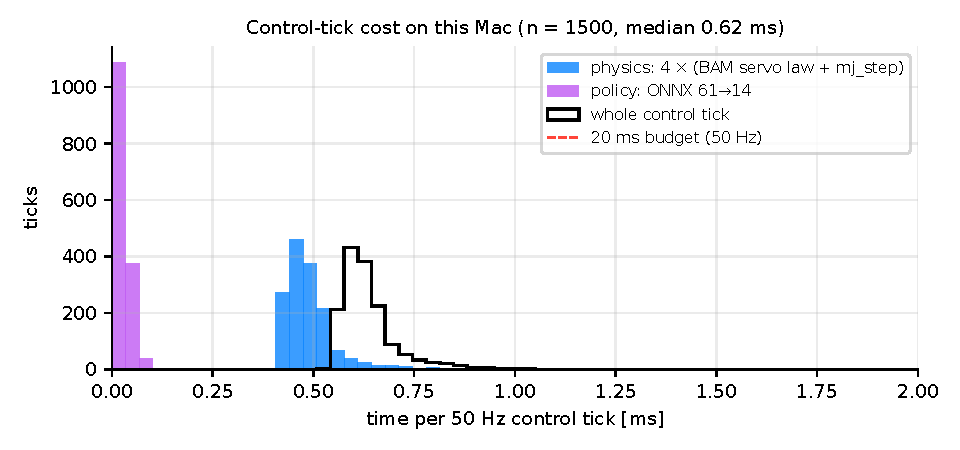
\includegraphics[width=0.7\linewidth]{figures/duck_app_step_time.pdf}
\caption{Control-tick cost on the Mac (M1~Max), split into physics (BAM law + \code{mj\_step}, $\times4$) and the ONNX
actor.}\label{fig:step}\end{figure}

\subsection{B. Speed tracking}\label{sec:exp:speed}
Each command is held for 6~s from a stand; the achieved speed is the trunk's forward velocity averaged over the
last 4~s, \speedTrials~trials per command (\fig{speed}, \tab{speed}). VelStand tracks every command of its band,
$-0.4$ to $0.6$~m/s, to within \walkMaxErr~m/s (it runs slightly fast, by 0.01--0.05~m/s), including $\pm0.1$~m/s
where the earlier walk export crouched and stood still; the trunk stays at 118--122~mm. Run~v3 tracks 0.3--0.7~m/s
with a growing deficit (\runTopAch~m/s at \runTopCmd), reaches 0.72~m/s at 0.8 with a wide spread, and falls at
\runFallCmds~m/s (at 1.0 and 1.1 the duck drops onto its belly). The run levels therefore stop at 0.8~m/s and the
top level is the sprint policy: \sprintAch~m/s (\sprintMin--\sprintMax over the trials), \sprintFalls~falls, trunk at
121~mm, the flight-phase gait at the servo speed limit that Newton measured at 1.1--1.2~m/s. Newton's evaluation of
run~v3 (\code{docs/run\_v3b\_speed\_5999\_*.json}) peaks at 0.63~m/s at the 0.9 command, so this plant lets the runner
go a little faster before it fails.
\begin{figure}[h]\centering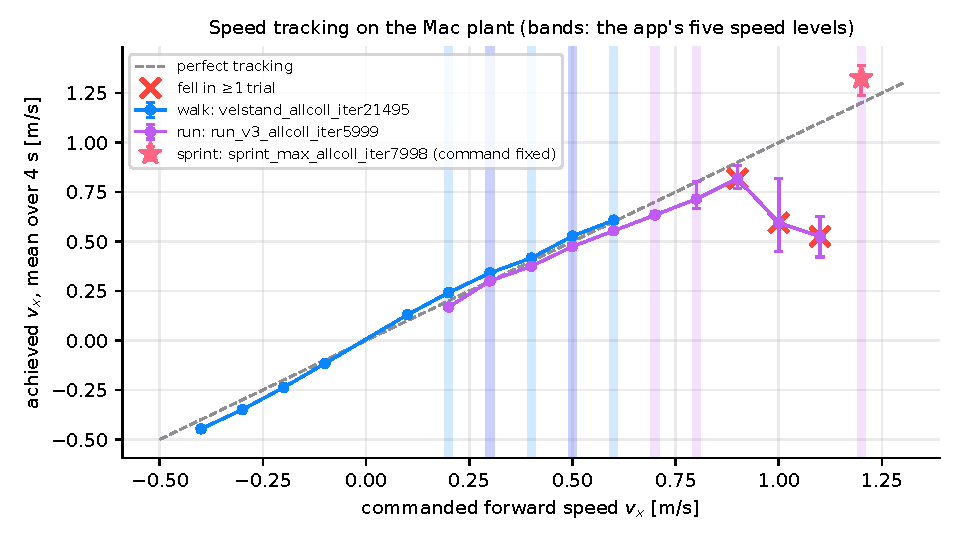
\includegraphics[width=0.7\linewidth]{figures/duck_app_speed_tracking.pdf}
\caption{Commanded against achieved forward speed; bars span the trials, bands mark the app's five speed levels
(the sprint's command is fixed at 1.2).}
\label{fig:speed}\end{figure}
\begin{table}[h]\centering\small\begin{tabular}{llrrrr}\toprule
policy & $v_x$ cmd [m/s] & achieved mean [m/s] & range over trials & trunk $z$ [mm] & falls \\\midrule
walk & -0.40 & -0.447 & [-0.456, -0.436] & 121 & 0/4 \\
walk & -0.30 & -0.350 & [-0.362, -0.337] & 120 & 0/4 \\
walk & -0.20 & -0.238 & [-0.240, -0.236] & 119 & 0/4 \\
walk & -0.10 & -0.117 & [-0.122, -0.110] & 118 & 0/4 \\
walk & +0.10 & +0.130 & [+0.127, +0.133] & 120 & 0/4 \\
walk & +0.20 & +0.242 & [+0.235, +0.249] & 121 & 0/4 \\
walk & +0.30 & +0.341 & [+0.339, +0.345] & 121 & 0/4 \\
walk & +0.40 & +0.416 & [+0.411, +0.420] & 121 & 0/4 \\
walk & +0.50 & +0.527 & [+0.521, +0.530] & 122 & 0/4 \\
walk & +0.60 & +0.608 & [+0.599, +0.613] & 122 & 0/4 \\
run & +0.20 & +0.169 & [+0.168, +0.170] & 118 & 0/4 \\
run & +0.30 & +0.301 & [+0.294, +0.309] & 119 & 0/4 \\
run & +0.40 & +0.375 & [+0.373, +0.376] & 121 & 0/4 \\
run & +0.50 & +0.475 & [+0.474, +0.475] & 121 & 0/4 \\
run & +0.60 & +0.554 & [+0.551, +0.557] & 121 & 0/4 \\
run & +0.70 & +0.634 & [+0.623, +0.650] & 121 & 0/4 \\
run & +0.80 & +0.715 & [+0.666, +0.803] & 120 & 0/4 \\
run & +0.90 & +0.817 & [+0.765, +0.882] & 117 & 1/4 \\
run & +1.00 & +0.595 & [+0.451, +0.818] & 110 & 3/4 \\
run & +1.10 & +0.524 & [+0.421, +0.626] & 106 & 4/4 \\
sprint & +1.20 & +1.327 & [+1.239, +1.388] & 121 & 0/4 \\
\bottomrule\end{tabular}

\caption{Speed tracking, all commands (mean over the last 4~s of 6; range over trials; mean trunk height).}\label{tab:speed}\end{table}

\subsection{C. Turning}\label{sec:exp:turn}
Turning in place (\fig{turn}, \tab{turn}): VelStand turns at every command, including the $\pm0.25$ and
$\pm0.5$~rad/s the earlier walk export ignored, and over-rotates by 25--50\% (1.0 commanded gives about
1.4~rad/s; largest error \turnMaxErr~rad/s). Turning while walking at 0.35~m/s under-tracks instead (0.27 and
0.36~rad/s for 0.5 and 0.85 commanded), so a curve at speed is wide. The yaw levels (0.5--0.8~rad/s) are chosen so a
turn in place runs at about 0.7--1.1~rad/s.
\begin{figure}[h]\centering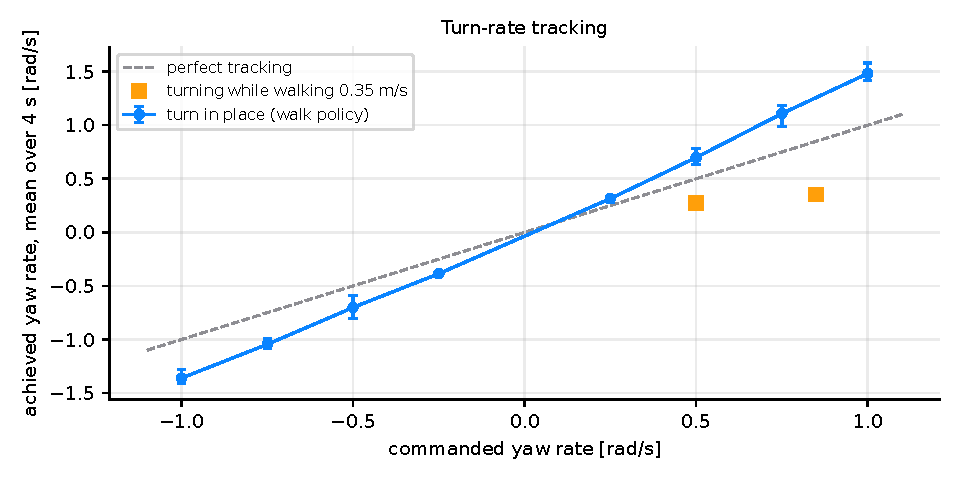
\includegraphics[width=0.7\linewidth]{figures/duck_app_turn_tracking.pdf}
\caption{Yaw-rate tracking in place and while walking.}\label{fig:turn}\end{figure}
\begin{table}[h]\centering\small\begin{tabular}{rrrr}\toprule
yaw cmd [rad/s] & achieved mean [rad/s] & range over trials & falls \\\midrule
-1.00 & -1.361 & [-1.409, -1.277] & 0/4 \\
-0.75 & -1.046 & [-1.082, -0.988] & 0/4 \\
-0.50 & -0.701 & [-0.806, -0.590] & 0/4 \\
-0.25 & -0.386 & [-0.411, -0.364] & 0/4 \\
+0.25 & +0.315 & [+0.283, +0.346] & 0/4 \\
+0.50 & +0.698 & [+0.637, +0.778] & 0/4 \\
+0.75 & +1.108 & [+0.987, +1.187] & 0/4 \\
+1.00 & +1.482 & [+1.420, +1.580] & 0/4 \\
\multicolumn{4}{l}{\emph{while walking 0.35 m/s}: yaw +0.50 $\to$ +0.272 rad/s, $v_x$ +0.379 m/s, falls 0/4} \\
\multicolumn{4}{l}{\emph{while walking 0.35 m/s}: yaw +0.85 $\to$ +0.355 rad/s, $v_x$ +0.383 m/s, falls 0/4} \\
\bottomrule\end{tabular}

\caption{Turn-rate tracking (\turnTrials~trials per command).}\label{tab:turn}\end{table}

\subsection{D. Transitions}\label{sec:exp:transitions}
\fig{trans}. \textbf{Stand.} VelStand at zero twist holds the trunk at \standZ~mm (minimum over trials
\standZmin~mm; the trained stand is 115--116~mm), so the idle duck no longer squats. \textbf{Sit.} After S the trunk
passes below 0.075~m after \sitSettleMean~s on average (\sitSettleMin--\sitSettleMax~s, \transTrials~trials) and rests
at \sitZ~mm, the trained seated height. \textbf{Stand up.} S again: $z>0.10$~m after \standUpMean~s
(\standUpMin--\standUpMax~s) in \standUpN/\transTrials~trials, final height \standUpZ~mm,
\standUpStanding/\transTrials~trials end in the \textsf{stand} state. The fast sit--stand replaces the 2~s
transitions (0.6--7.5~s stand-up on this plant) of the earlier export; the earlier finding stands that targets must
not be clipped to the joint range, or the knee stalls $17^\circ$ short of its limit and the duck never rises.
\textbf{Stop.} Releasing the keys at every level of every gait (\tab{stop}) ends in the stand state with
$|v_x|<0.03$~m/s within \stopMaxS~s and \stopMaxM~m at most, \stopFalls/\stopTrials~falls---the one fall is a stop
from the sprint, where the hand-over from a 1.3~m/s flight gait to VelStand occasionally lands the duck on its
head, and VelStand then gets up. \textbf{Hot swap.} walk$\to$run$\to$walk at level~3 with the shared last-action
buffer: \handoverFalls/\handoverTrials~falls; walk$\to$sprint$\to$walk at level~5:
\sprintHandoverFalls/\sprintHandoverTrials.
\begin{figure}[h]\centering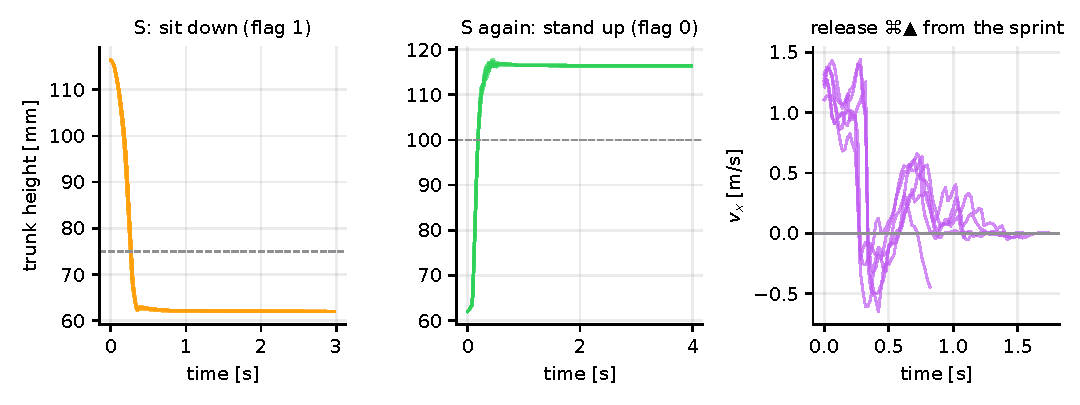
\includegraphics[width=0.85\linewidth]{figures/duck_app_transitions.pdf}
\caption{Trunk height while sitting down and standing up (all trials), and forward speed after releasing
\cmdkey$\blacktriangle$ from the sprint.}\label{fig:trans}\end{figure}
\begin{table}[h]\centering\small\begin{tabular}{llrrrr}\toprule
level & gait & $v_x$ cmd [m/s] & time to stand, mean (max) [s] & distance, mean (max) [m] & falls \\\midrule
1 & walk & 0.20 & 0.77 (0.82) & 0.06 (0.06) & 0/6 \\
1 & run & 0.30 & 1.04 (1.14) & 0.15 (0.20) & 0/6 \\
2 & walk & 0.30 & 0.85 (0.90) & 0.08 (0.09) & 0/6 \\
2 & run & 0.50 & 1.11 (1.22) & 0.22 (0.28) & 0/6 \\
3 & walk & 0.40 & 0.93 (0.96) & 0.11 (0.12) & 0/6 \\
3 & run & 0.70 & 1.26 (1.32) & 0.30 (0.33) & 0/6 \\
4 & walk & 0.50 & 1.02 (1.12) & 0.16 (0.18) & 0/6 \\
4 & run & 0.80 & 1.44 (1.82) & 0.46 (0.67) & 0/6 \\
5 & walk & 0.60 & 1.10 (1.14) & 0.21 (0.22) & 0/6 \\
5 & sprint & 1.20 & 1.43 (1.76) & 0.48 (0.56) & 1/6 \\
\bottomrule\end{tabular}

\caption{Stopping from each speed level: time from key release to a standing duck, and distance covered.}\label{tab:stop}\end{table}

\subsection{E. Jump}\label{sec:exp:jump}
Space from a jittered stand, \jumpN~trials (\fig{jump}). Take-off in \jumpTakeoff/\jumpN; the trunk rises
\jumpRiseMean~mm on average (\jumpRiseMin--\jumpRiseMax), the flight lasts \jumpAirMean~ms, touchdown comes 0.32--0.36~s
after the press, and the walk policy has the stand back after \jumpBackMean~s (\jumpBackMax at most);
\jumpStanding/\jumpN~trials are standing one second later, \jumpFell~went to the floor. Newton measured the same
checkpoint at 83\% take-off and 30~mm; the hop is the servo ceiling, not a tuning choice. The hand-back window is
the one result of this section that is a plant finding rather than a confirmation: left running after the landing
(as the training episode does for 3~s), the jump policy holds its landing only 0.3--0.5~s and then drifts forward
and tips over on this plant---10/12 trials with a 1~s quiet window, 1/12 with 0.3~s, 0/12 with 0.1~s---so the walk
policy takes the stand over as soon as the landing is quiet. On the robot the same logic applies: the jump is a
one-shot behaviour and VelStand owns the stand.
\begin{figure}[h]\centering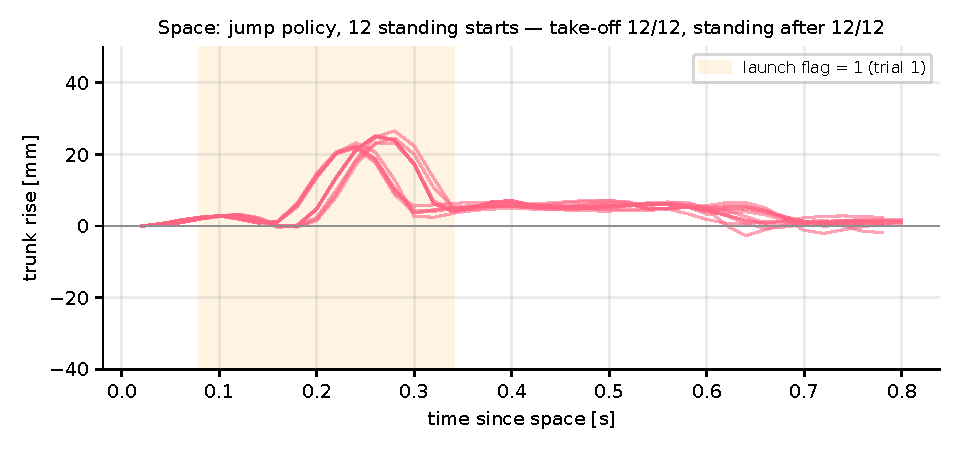
\includegraphics[width=0.7\linewidth]{figures/duck_app_jump.pdf}
\caption{Trunk rise after space for all trials; the shaded band is the launch flag of the first trial.}\label{fig:jump}\end{figure}

\subsection{F. Front flip}
R from a jittered stand, \rollN~trials (\fig{roll}): the duck rolls \rollDegMean$^\circ$ about its pitch axis
(\rollDegMin--\rollDegMax$^\circ$), is upright again \rollUpMean~s after the press (\rollUpMax at most) and
\rollStanding/\rollN~trials end standing under the walk policy; \rollFell~needed the stand-up policy
(\rollCompleted/\rollN completed the roll). The policy is \code{\polRoulade}, the straight-head fine-tune that
replaced \code{roulade\_iter6000} on 2026-11-16: in Newton it ends with the head 3.7$^\circ$ from home instead of
57.6$^\circ$, completes the roll and stands in 90.6\% of 96 trials and ends standing in all of them (the earlier
export: 96.9\% landed standing). This plant reproduces the behaviour without a failure in the sample from a quiet
stand; in the keyboard scenario of \S\ref{sec:exp:seq}, where the flip follows a jump, one of eight ended on the
floor.
\begin{figure}[h]\centering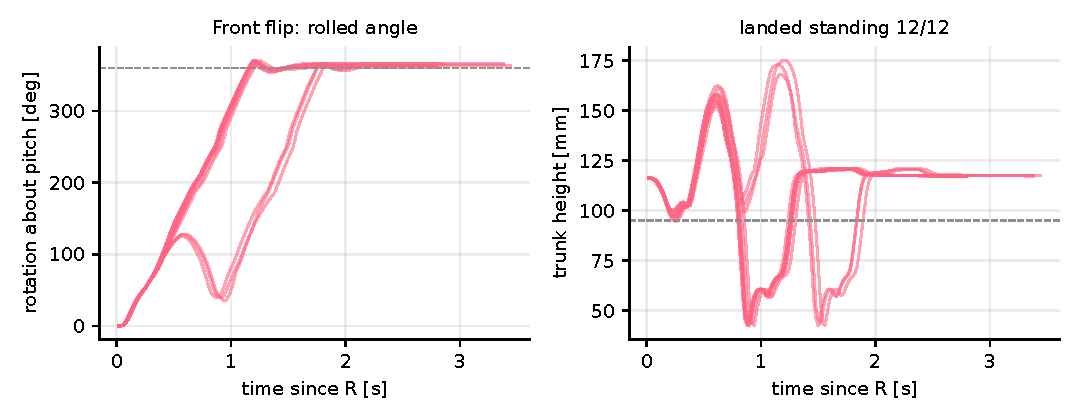
\includegraphics[width=0.85\linewidth]{figures/duck_app_roulade.pdf}
\caption{Front flip: integrated pitch rotation and trunk height for all trials.}\label{fig:roll}\end{figure}

\subsection{G. Pushes and getting up}\label{sec:exp:recovery}
\fig{recovery}, \tab{push}, \tab{getup}. \textbf{Pushes}: the training's disturbance (a horizontal velocity
impulse of \pushLevels~m/s added to the trunk in a random direction, \code{scripts/push\_test.py}), \pushRepeats~per
level, in four conditions: standing and walking at 0.3~m/s under VelStand with the fall left to VelStand; walking
with every fall routed to the stand-up policy; and running at 0.7~m/s (run~v3 cannot recover, so the stand-up
policy takes over). A fall is tilt $>60^\circ$ within the 2~s after the push; ``upright after 2~s'' is tilt
$<20^\circ$ and $z>0.095$~m at that moment, the test of the repository's push evaluation. Standing VelStand is
toppled from 1.0~m/s on in about half the pushes and is back on its feet 0.6--0.7~s later every time; walking it
falls from 1.5--2.0~m/s on and is upright again within 2~s in all but one push (at 2.0~m/s, the one case not
upright at the 2~s mark); routed to the stand-up policy instead, every fall while walking was recovered, 0.8--1.3~s
after the fall; running, every push of 1.0~m/s or more fells the duck and the stand-up policy brought it back in
every case, 0.9--1.4~s after the fall. Every condition was upright after 2~s for all pushes up to
\pushAllUpright~m/s; over all conditions \pushRecovered/\pushFallsTotal~falls were recovered within the window.
\textbf{Get-up battery}: the duck is dropped prone (face down), supine (face up) or on a side with $\pm10^\circ$ of
noise and $\pm0.1$~rad on the joints, settles for 1~s with the servos holding the default pose, then one policy runs
at zero twist: \getupSuccess/\getupTrials~successes, upright within \getupMaxS~s at most; VelStand and the stand-up
policy take 0.4--0.6~s from prone and supine, VelStand a little longer from the side. On this plant the two are
equivalent for getting up; the stand-up policy is kept as the recovery role because it is the one that was
trained to \emph{hold} a stand afterwards, and because the run, sprint, sit and trick policies cannot recover.
\begin{figure}[h]\centering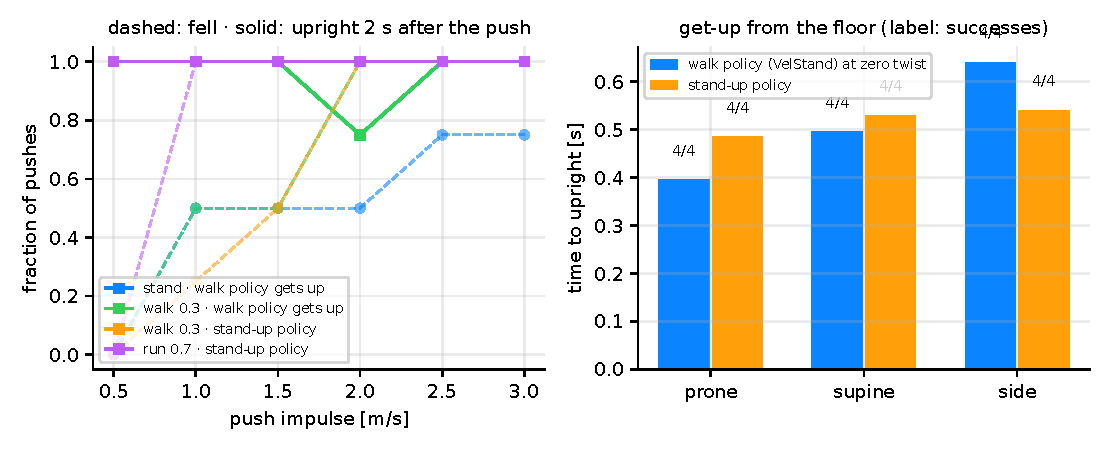
\includegraphics[width=0.85\linewidth]{figures/duck_app_recovery.pdf}
\caption{Left: fraction of pushes that felled the duck (dashed) and that left it upright 2~s later (solid), per
condition. Right: time to upright from the floor, with successes.}\label{fig:recovery}\end{figure}
\begin{table}[h]\centering{\footnotesize\setlength{\tabcolsep}{3.5pt}\begin{tabular}{lcccccc}\toprule
condition & 0.5 m/s & 1.0 m/s & 1.5 m/s & 2.0 m/s & 2.5 m/s & 3.0 m/s \\\midrule
stand, walk policy gets up & 0 / 4 & 2 / 4 & 2 / 4 & 2 / 4 & 3 / 4 & 3 / 4 \\
walk 0.3, walk policy gets up & 0 / 4 & 2 / 4 & 2 / 4 & 4 / 3 & 4 / 4 & 4 / 4 \\
walk 0.3, stand-up policy & 0 / 4 & 1 / 4 & 2 / 4 & 4 / 4 & 4 / 4 & 4 / 4 \\
run 0.7, stand-up policy & 0 / 4 & 4 / 4 & 4 / 4 & 4 / 4 & 4 / 4 & 4 / 4 \\
\bottomrule\end{tabular}
}
\caption{Pushes: fell $\cdot$ upright after 2~s, out of \pushRepeats~per level.}\label{tab:push}\end{table}
\begin{table}[h]\centering\small\begin{tabular}{llrrr}\toprule
get-up policy & start pose & upright & time to upright, mean [s] & max [s] \\\midrule
walk policy (VelStand) at zero twist & prone & 4/4 & 0.40 & 0.40 \\
walk policy (VelStand) at zero twist & supine & 4/4 & 0.49 & 0.52 \\
walk policy (VelStand) at zero twist & side & 4/4 & 0.64 & 0.78 \\
stand-up policy & prone & 4/4 & 0.48 & 0.74 \\
stand-up policy & supine & 4/4 & 0.53 & 0.54 \\
stand-up policy & side & 4/4 & 0.54 & 0.58 \\
\bottomrule\end{tabular}

\caption{Get-up from the floor (hand-back wait excluded).}\label{tab:getup}\end{table}

\subsection{H. The keyboard scenario}\label{sec:exp:seq}
The sequence a user would type---stand, $\blacktriangle$ 4~s, \cmdkey$\blacktriangle$ 4~s, release, S (sit)
2~s, S (stand) 2~s, $\blacktriangleleft$ 4~s, $\blacktriangle$+$\blacktriangleright$ 4~s, $\blacktriangledown$ 3~s,
\optkey$\blacktriangleleft$ 3~s, release, space 3~s, R 4~s, D~D then \cmdkey$\blacktriangle$ (sprint) 4~s,
release---\seqSegments~segments over \seqTrials~jittered starts: \seqClean/\seqTrials~clean, \seqFalls~falls in
total, \seqDist~m covered per run on average, every run ending in the stand state. Three of the four falls were
the last segment, the stop from the sprint (the failure mode of \S\ref{sec:exp:transitions}), and VelStand was
back on its feet before the segment ended; the fourth was the front flip of one run, which ended on the floor and
was stood up by the stand-up policy. The jump never fell in the scenario.

\section{Implementation and usage}
\begin{verbatim}
app/setup.sh                  # once: ~/.venvs/microduck_live (MuJoCo, ORT, BAM)
app/ducklive.sh               # open /Applications/Duck Live.app (built once)
app/ducklive.sh --browser | --serve | --install-app | --sync
app/sync_policies.sh --local  # git pull + repack sidecar exports
app/bench_mac.py              # this document's numbers -> figures, *_table.tex
\end{verbatim}
The window starts \code{app/server.py} with the venv's Python, waits for its \code{DUCK\_LIVE\_READY <port>
<token>} line and loads \code{http://127.0.0.1:<port>/?token=\ldots\&native=1}; the token guards every API and
the WebSocket, so no other local page can drive the duck. Policies are the files in \code{exports/} matched to the
roles of \tab{roles}; the \gear panel swaps any role (the optional ones can be switched off), routes falls to the
stand-up policy, and changes the plant parameters (delay, supply, sag) at run time. \code{--sync} runs
\code{git pull}, repacks exports whose weights sit in a sidecar, and copies newer exports from the 5080 over
\code{ssh 5080} (repacking those too). Nothing here touches the real robot: deployment stays \code{robotctl policy
load} with the same ONNX files, and the operator logic of \S\ref{sec:operator}---including the jump's launch-flag
protocol and the fall routing---is what a gamepad mapping on the robot would do.

\section{Limitations}\label{sec:lim}
\begin{itemize}[nosep]
\item \textbf{Plant mismatch.} C~MuJoCo here, Newton/MJWarp in training. Run~v3 goes faster here before it fails
  (0.72~m/s at 0.8 against Newton's 0.63 peak), VelStand over-rotates in place, and the jump policy's landing hold
  is shorter than its training episode. Success rates in this document are for this plant.
\item \textbf{No sensor noise, no IMU misalignment, no encoder bias, no dropout} at inference---the policies see
  clean observations, as in the repository's own evaluations. A ``realism'' toggle is a small addition.
\item \textbf{Fixed delay and supply} in the app ($L=4$, 7.7~V, sag 0.1); the measurements draw $L$ but not the
  supply. The \gear panel changes them, which rebuilds the plant.
\item \textbf{Run and sprint go straight.} Both recipes command no yaw; turning while \cmdkey is held is ignored
  (the HUD says so). A run policy with yaw is the obvious next export.
\item \textbf{Stopping from the sprint} is the one transition that can end on the floor (1 in 6 here); VelStand
  gets up, but a dedicated deceleration behaviour, or a sprint fine-tuned with a zero-command share, would remove it.
\item \textbf{The jump is a 2--3~cm hop} and the hand-back is immediate because the landing hold is not reliable
  here; a jump recipe fine-tuned with a longer post-landing hold on this plant would let the jump policy own its
  landing.
\item \textbf{Browser mode} (\code{--browser}) cannot see a key-up while \cmdkey is held; the page clears the
  held keys when \cmdkey is released, so the duck stops a moment late. The app window does not have the issue.
\end{itemize}

\begin{thebibliography}{9}
\bibitem{mujoco} E.~Todorov, T.~Erez, Y.~Tassa. MuJoCo: A physics engine for model-based control. IROS, 2012.
\bibitem{bam} M.~Duclusaud, G.~Passault, V.~Padois, O.~Ly. Extended friction models for the physics simulation of
  servo actuators. arXiv:2410.08650, 2024. \url{https://github.com/Rhoban/bam}
\bibitem{isaaclab} M.~Mittal et al. Orbit: A unified simulation framework for interactive robot learning
  environments. IEEE RA-L, 2023 (Isaac Lab). \url{https://github.com/isaac-sim/IsaacLab}
\bibitem{rudin} N.~Rudin, D.~Hoeller, P.~Reist, M.~Hutter. Learning to walk in minutes using massively parallel deep
  reinforcement learning. CoRL, 2021 (RSL-RL).
\bibitem{ppo} J.~Schulman, F.~Wolski, P.~Dhariwal, A.~Radford, O.~Klimov. Proximal policy optimization algorithms.
  arXiv:1707.06347, 2017.
\bibitem{microduck} Pollen Robotics. Microduck: a tiny biped duck robot, and \code{microduck\_rl} (VelStand,
  StandUp, Roulade recipes). \url{https://github.com/pollen-robotics/microduck}
\bibitem{hfblog} NVIDIA and Hugging Face. Train in simulation, deploy on a real robot: Microduck with Isaac Lab
  3.0. 2026. \url{https://huggingface.co/blog/nvidia/microduck-isaac-lab-sim-to-real}
\bibitem{mjwarp} Google DeepMind and NVIDIA. MuJoCo Warp (MJWarp). 2025. \url{https://github.com/google-deepmind/mujoco_warp}
\bibitem{jumpref} T.~Burgess. microduck-max-height-jump (community jump recipe, v6), 2026.
  \url{https://github.com/ThomasBurgess2000/microduck-max-height-jump}
\end{thebibliography}
\end{document}
